\documentclass[12pt,twoside]{article}
\usepackage{jmlda}
\bibliographystyle{utf8gost705u}
%\NOREVIEWERNOTES
\title
    [Обучение машинного перевода без параллельных текстов] % Краткое название; не нужно, если полное название влезает в~колонтитул
    {Обучение машинного перевода без параллельных текстов}
\author
    [Артеменков$^1$~А.\,А., Бахтеев$^1$~О.\,Ю., Стрижов$^2$~В.\,В.] % список авторов для колонтитула; не нужен, если основной список влезает в колонтитул
    {Артеменков$^1$~А.\,А., Бахтеев$^1$~О.\,Ю., Стрижов$^2$~В.\,В.} % основной список авторов, выводимый в оглавление
    [Артеменков$^1$~А.\,А., Бахтеев$^1$~О.\,Ю., Стрижов$^2$~В.\,В.] % список авторов, выводимый в заголовок; не нужен, если он не отличается от основного
\thanks
    {Научный руководитель:  Стрижов~В.\,В. 
   Авторы: А.В. Грабовой, О.Ю. Бахтеев, В.В. Стрижов, Eric Gaussier, координатор Малиновский~Г.\,С.
   Консультант:  Бахтеев~О.\,Ю.}
%\email
%    {author@site.ru}
\organization
{$^1$Московский физико-технический институт\par
	$^2$Вычислительный центр им. А.~А. Дородницына ФИЦ ИУ РАН}
\abstract
    {В данной работе исследуется задача машинного перевода между двумя языками. Предлагается подход, основанный на моделях автокодировщиков и не требующий наличия большого корпуса параллельных предложений. Каждому предложению из обоих языков ставится в соответствие представление в общем скрытом пространстве. Оптимизация проводится таким образом, чтобы скрытые пространства автокодировщиков для разных языков совпадали. Для проверки качества модели проводится вычислительный эксперимент по переводу предложений между парой языков русский-украинский. 

\bigskip
\textbf{Ключевые слова}: \emph {нейронные сети, машинный перевод, автокодировщики}.}
\begin{document}
\maketitle

\section{Введение}

Целью данной работы является  ьрешение задачи машинного перевода в отсутствии достаточного корпуса параллельных предложений. При наличии нескольких миллионов \cite{bahdanau2014neural} параллельных образцов хорошо себя показывают методы машинного перевода с использованием нейронных сетей \cite{cho2014properties}, \cite{luong2015effective}. Высокие результаты достигаются при использовании глубоких (свёрточных или рекуррентных) нейронных сетей, однако, в данном подходе критично наличие большой обучающей выборки. Частичное решение данной проблемы было найдено в пополнении числа предложений с помощью использования переводчиков более низкого качества. В \cite{bertoldi2009domain} было показано, что данным способом могут быть улучшены результаты работы системы статистического машинного перевода Moses \cite{koehn2007moses}. Более общим подходом является отказ от перевода в одну сторону и параллельное обучение переводчиков таким образом, чтобы один пополнял обучающую выборку другого.

Описанный выше метод был использована в \cite{lample2017unsupervised} для перевода предложений с английского языка на французский. В данной работе подобная технология будет применяться для перевода с русского языка на украинский. Рассматриваются автокодировщики, реализованные в виде рекуррентных нейронных сетей \cite{gers1999learning}, \cite{graves2005framewise}, используемые для прямого и обратного перевода, и сеть-дискриминатор, оптимизируемая с целью по представлению слова в векторном пространстве определять язык \cite{goldberg2014word2vec}. Автокодировщики оптимизируются таким образом, чтобы их латентные представления совпадали, или, что эквивалентно, чтобы дискриминатор не мог с достаточной уверенностью определить язык, соответствующий сгенерированному вектору. Для того, чтобы избежать переобучения, добавляется шум, не дающий автокодировщикам восстанавливать предложения в точности. Шаг оптимизации состоит из двух стадий: оптимизация дискриминатора и оптимизация переводчика. На первой стадии выбирается случайное предложение из исходного языка, кодируется с добавлением шума \cite{kimimproving}) и подаётся на вход дискриминатору. После шага оптимизации аналогичные действия повторяются со случайным предложением из конечного языка. На второй стадии выбирается случайное предложение из исходного языка и переводится текущей версией переводчика на конечный язык. Затем на него накладывается шум, оно кодируется, и считываются показания дискриминатора. После шага оптимизации предложение переводится обратно в исходный язык и вычисляется значение функции потерь. После шага оптимизации действия повторяются со случайным предложением из конечного языка. 

В качестве эксперимента производится перевод предложений с русского языка на украинский. Для этой пары языков отсутствует большие выборки параллельных предложений в открытом доступе, при этом достаточно данных по каждому из языков в отдельности. Качество полученного в результате переводчика оценивается с помощью метрики BLEU \cite{papineni2002bleu}. 

\section{Постановка задачи}

Введём индекс $l \in \{\text{src}, \text{tgt}\}$, показывающий, к какому языку относится рассматриваемый объект. Обозначим через $\mathfrak{D}^{l} = [\mathbf{s}_1^{l}, \dots, \mathbf{s}_{m_l}^{l}]$ корпус предложений со словарём $V^{l} = \{w_i^{l}\}_{i=1}^{|V^{l}|}$. В общем случае, корпуса $\mathfrak{D}^{\text{src}}$ и $\mathfrak{D}^{\text{tgt}}$ не являются параллельными. Валидационная выборка, состоящая из параллельных предложений, далее будет обозначаться как $\mathfrak{D}^{valid} = \{(\mathbf{s}_1^{\text{src}}, \mathbf{s}_1^{\text{tgt}}), \dots, (\mathbf{s}_{m_\text{valid}}^{\text{src}}, \mathbf{s}_{m_\text{valid}}^{\text{tgt}})\}$. Обозначим пространство предложений как $\mathcal{S}^{l}$, где каждое предложение есть набор слов: $\mathbf{s}_i^{l} = \{w_k\}_{k=1}^{|\mathbf{s}_i^{l}|}$. Введём в рассмотрение скрытое пространство $\mathcal{Z}$, общее для обоих языков, элементами которого являются коды предложений: $\{\mathbf{z}_i\}_{i=1}^k, \mathbf{z}_i \in \mathbb{R}^h$. Количество $k$ векторов в скрытом представлении совпадает с числом слов исходного предложения и для разных предложений может отличаться. 

В процессе оптимизации параметров модели каждое слово предложения представляется в виде вектора вероятностей $\mathbf{p} \in \mathbb{R}^{|V^{l}|}, \; \sum_{i=1}^{V^{l}} p_i = 1, \; p_i \ge 0$, где $p_i$ есть вероятность появления слова $w_i^{l} \in V^{l}$ на данной позиции. Рассматриваемая модель состоит кодировщика $\mathbf{f}^{l}: \; \mathcal{S}^l \to \mathcal{Z}$ и декодировщика $\mathbf{g}^l: \; \mathcal{Z} \to \mathcal{S}^l$, отвечающих соответственно за отображение предложений из обоих языков в общее латентное пространство $\mathcal{Z}$ и обратное отображение из пространства $\mathcal{Z}$ в предложения первого или второго языка. Параметры как кодировщиков $\mathbf{f}^{\text{src}}$ и $\mathbf{f}^{\text{tgt}}$, так и декодировщиков $\mathbf{g}^{\text{src}}$ и $\mathbf{g}^{\text{tgt}}$ являются общими. Для обоих языков отличается лишь часть модели, генерирующая вектор вероятностей $\mathbf{p}$ по состоянию декодировщика.

 Максимизируется следующая функция качества:

\[ L = \frac{1}{m_\text{valid}} \sum_{i=1}^{m_\text{valid}} \text{BLEU}(g^{\text{tgt}}(f^{\text{src}}(\mathbf{s}_{i}^{\text{src}})), \; \mathbf{s}_{i}^{\text{tgt}})\]

Отсутствие параллельных предложений в обучающей выборке можно компенсировать с помощью сходства латентных пространств. В данной работе для этого предпринимаются следующие действия:
\begin{enumerate}
	\item 
	используется сеть-дискриминатор $\mathbf{discr}$, которая по латентному представлению $\mathbf{z}$ предложения $\mathbf{s}$ определяет, какому языку оно принадлежит;
	\item
	функция потерь записывается таким образом, чтобы оптимизировать дискриминатор $\mathbf{discr}$ для верного распознавания языка предложения, а автокодировщик -- для генерации похожих представлений предложений из разных языков;
	\item 
	во избежание переобучения, каждый раз перед кодированием предложения к нему добавляется шум $\sigma(\cdot)$: из предложения опускаются некоторые слова, а к оставшимся применяется перестановка $\pi$ таким образом, чтобы слова переставлялись не слишком далеко: $\max (\pi(i)-i) \le k$. 
\end{enumerate}
 
 Обозначим через $\mathbf{s}(k)$ вектор вероятностей $\mathbf{p}$, соответствующий $k$-му слову предложения $\mathbf{s}$. В качестве метрики между словами предлагается использовать $\text{NLL}(\cdot, \cdot)$ (negative log likelihood).
 
 \[ \text{NLL}(w_i^l, \mathbf{p}) = -\sum_{k=1}^{|V^{l}|} \mathbb{I}\{k = i\} \log p_k\]
 
 Введём обозначение для противоположного языка: $\widehat{l} = \text{src}$, если $l = \text{tgt}$, и $\widehat{l} = \text{tgt}$, если $l = \text{src}$. Функции потерь для переводчика $L$ и дискриминатора $L_{D}$ записываются следующим образом:
 
 \[ L = aL_{AE} + bL_{TR} + cL_{ADV} \]
 
 \begin{enumerate}
 	\item \textit{Ошибка автокодировщика}
 	
 	Отвечает за правильное восстановление зашумлённых предложений из латентного пространства.
 	\[ L_{AE} = \sum_{k=1}^{|\mathbf{s}^l|}\text{NLL}(\mathbf{g}^l(\mathbf{f}^l(\sigma(\mathbf{s}^l)))(k), \mathbf{s}^l(k)) \]
 	
 	\item \textit{Ошибка перевода}
 	
 	Отвечает за качество перевода с использованием автокодировщиков.
 	\[ L_{TR} = \sum_{k=1}^{|\mathbf{s}^l|}\text{NLL}(\mathbf{g}^{\widehat{l}}(\mathbf{f}^l(\sigma(\mathbf{s}^l)))(k), \mathbf{s}^l(k)) \]
 	
 	\item \textit{Штраф на различие скрытых пространств}
 	
 	Отвечает за то, чтобы латентные пространства обоих автокодировщиков были похожи. Здесь же рассматривается ошибка дискриминатора $L_D$, показывающая, насколько точно определяется язык предложения по его скрытому представлению.
 	\[ L_{ADV} = -\log \mathbb{P}\{\mathbf{discr}(\mathbf{f}^l(\mathbf{s}^l)) = \widehat{l}\}\]
 	\[ L_{D}   = -\log \mathbb{P}\{\mathbf{discr}(\mathbf{f}^l(\mathbf{s}^l)) = l\}\]
 \end{enumerate}

\section{Базовый алгоритм}

В качестве нулевого приближения используется модель пословного перевода. Каждое предложение пословно заменяется на ближайшего по косинусному расстоянию соседа из векторного представления MUSE \cite{conneau2017word}. Этот перевод обладает не очень высоким качеством, так как не учитывает особенности построения предложений в разных языках. Однако, после применения шума, в нём оказываются и правильно переведённые предложения. За счёт этого оптимизируемая модель имеет возможность научиться строить переводы, которые отсутствовали в нулевом приближении. 

Кодировщик $\mathbf{f}^l$ является двунаправленной рекуррентной нейронной сетью GRU, декодировщик представляет собой GRU с сетью внимания и многослойную нейронную сеть, осуществляющую генерацию вектора вероятностей $\mathbf{p}$ по выходу GRU. Сеть внимания реализована с помощью однослойной нейронной сети, а дискриминатор -- многослойной нейронной сети. Перед подачей на вход кодировщику все слова в предложении заменяются на их векторное представление, которое инициализируется векторами MUSE и оптимизируется вместе с другими параметрами.

Алгоритм оптимизации может быть записан следующим образом:
\begin{enumerate}
	\item Построить нулевое приближение переводчика $M$
	\item Пока не достигнуто желаемое качество перевода:
	\begin{enumerate}
	\item Сделать $T$ шагов соревновательной оптимизации:
	\begin{enumerate}
		\item Вычислить $L$ и $L_D$
		\item Обновить параметры автокодировщиков с помощью градиентного спуска для $L$ при фиксированных параметрах дискриминатора
		\item Обновить параметры дискриминатора с помощью градиентного спуска для $L_D$ при фиксированных параметрах автокодировщиков
	\end{enumerate}
	\item Обновить $M$, записав в него переводчик, полученный из последовательного применения кодировщика и декодировщика
	\item Построить новый перевод обучающей выборки с использованием $M$
	\end{enumerate}
\end{enumerate}

\section{Вычислительный эксперимент}

В качестве обучающей выборки использовались данные Multi30k \cite{elliott-EtAl:2017:WMT}, \cite{W16-3210}. Параметры автокодировщиков оптимизировались с помощью Adam, параметры дискриминатора -- с помощью RMSprop.

\begin{figure}[h]
	\centering
	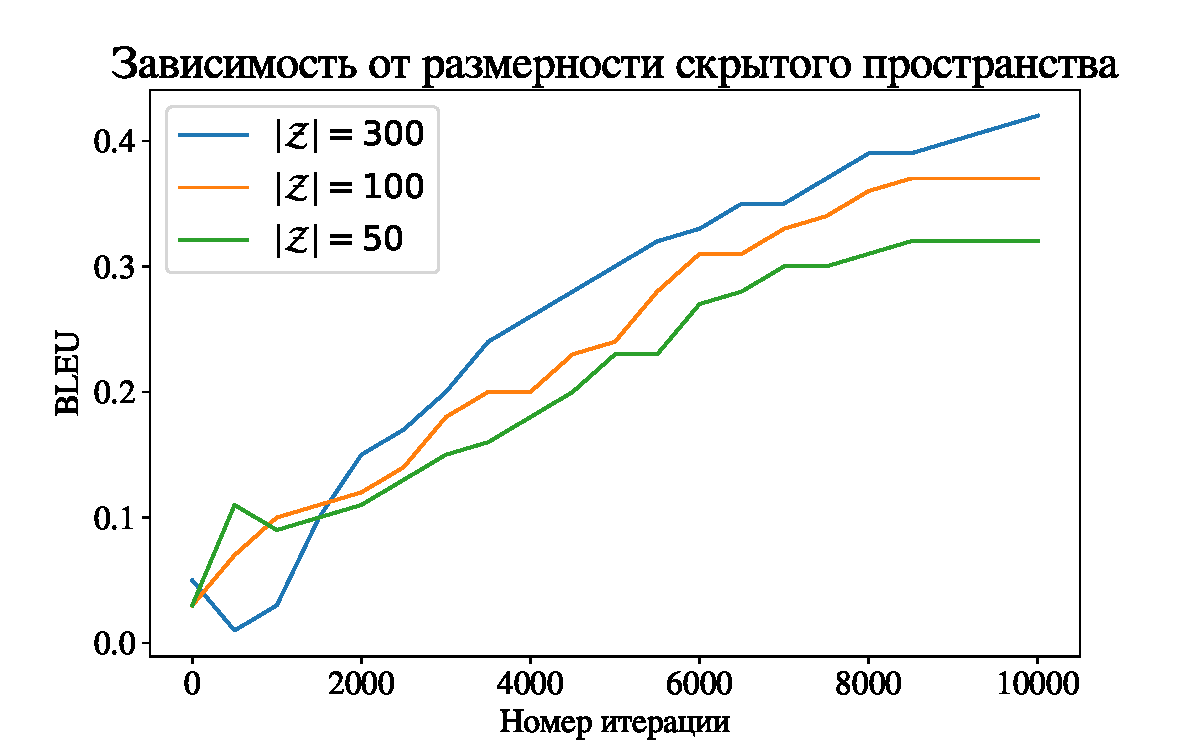
\includegraphics[width=0.7\textwidth]{hidden}
	\caption{Зависимость BLEU от номера итерации в зависимости от размерности скрытного пространства.}
\end{figure}

\section{Вывод}

В данной работе была исследована задача машинного перевода между двумя языками. Предложен подход, основанный на моделях автокодировщиков и не требующий наличия большого корпуса параллельных предложений. Работа была проделана на англо-французской выборке, так как качество найденных русско-украинских выборок не является достаточным как для построения хорошей модели, так и для валидации: в предложениях присутствует слишком много слов не из словаря (числа и формы слов), а сами переводы не всегда точны. Возможна дальнейшая работа по модификации алгоритма таким образом, чтобы это не так сильно влияло на качество перевода \cite{irvine2016end}, \cite{klementiev2012toward}. В данных работах предлагается извлечь дополнительную информацию из выборки для одного языка, что позволит сохранить независимость метода от наличия параллельных предложений.
\bibliography{references}

%\linenumbers

% Решение Программного Комитета:
%\ACCEPTNOTE
%\AMENDNOTE
%\REJECTNOTE
\end{document}
